%
%  hume.one
%
%  Created by Mark Eli Kalderon on 2007-07-28.
%  Copyright (c) 2007 Mark Eli Kalderon. All rights reserved.
%
%  Beamer

% Definitions and macros
\newcommand{\change}{\textcolor{blue}{\textbf{CHANGE SLIDE}}}
\newcommand\myauthor{Mark Eli Kalderon} 
\newcommand\mytitle{Introduction to Moral Philosophy}
\newcommand\mysubtitle{Hume}
\newcommand\myinstitution{University College London}
\newcommand\myurl{http://markelikalderon.com/teaching/}

% Packages specific to lecture notes
\mode<article>{
    \usepackage{palatino}
}

% Packages specific to beamer presentation
\mode<presentation>{
    \usetheme{Darmstadt}
    \setbeamercovered{transparent}
    \pgfdeclareimage[height=0.5cm]{university-logo}{../../../graphics/logo_sml_blk}
    \logo{\pgfuseimage{university-logo}}
}

% Packages common to lecture notes and beamer presentation
\usepackage{pgf}
\usepackage{tikz}
\usepackage{hyperref}

\setjobnamebeamerversion{hume.one.beamer}

\title{\mytitle}
\subtitle{\mysubtitle}

\author{\myauthor\\
\url{\myurl}}
\institute{\myinstitution}

% \date[Short Occasion] % (optional)
% {Date / Occasion}

\begin{document}

% TODO: Add CHANGE SLIDEs throughout

\frame{\maketitle}

\section{Overview}\label{sec:overview} % (fold)

\change\ The aim of these lectures is to introduce the student to the central themes of moral philosophy through the close examination of three key historical texts:
\begin{itemize}
    \item Book \textsc{iii} of David Hume's \emph{Treatise of Human Nature}
    \item Immanuel Kant's \emph{Groundwork for the Metaphysics of Morals}
    % \item Friedrich Nietzsche's \emph{On the Genealogy of Morals}
\end{itemize}
The objective is to provide the student with an in depth understanding of these texts and to provide the student with sufficient background for further study of both the texts under study and moral philosophy more generally.

I am loathe to recommend any secondary literature. The secondary literature on these topics is both vast and difficult, and, for now, students should spend their time and energy trying to understand Hume and Kant rather than trying to understand their commentators. However, if extra guidance is required, I would recommend two books:
\begin{itemize}
    \item John Rawls' \emph{Lectures on the History of Moral Philosophy}
    \item David Wiggins' \emph{Ethics: Twelve Lectures on the Philosophy of Morality}
\end{itemize}
Both books are based on a course of lectures like this one, and both lecture series had the same basic aim---to introduce moral philosophy through the close reading of key hostorical texts. There are crucial differences, however. My interpretation of Hume and Kant does not always conform to the interpretation they give (and their interpretations are not always consistent with one another). So whom should you trust? Well, as always, only the historical text is truly authoritative. These lectures and the secondary literature that I have recommended are merely aids to your reading of these texts. It is Hume, Kant, and Nietzsche who should have the final say concerning the content of their doctrines. \change

% \textbf{See Figure~\ref{fig:slide1}.}
% 
% \begin{figure}[ht]
%     \begin{center}
%         \includeslide[height=5cm]{slide1<1>}
%     \end{center}
%     \caption{Introduction to Ethics}
%     \label{fig:slide1}
% \end{figure}

\frame<presentation>[label=slide1]{
    \frametitle{Introduction to Ethics}
        \alert{Main Reading:}
            \begin{itemize}
                \item David Hume, Book III of the \emph{Treatise of Human Nature}
                \item Immanuel Kant, \emph{Groundwork for the Metaphysics of Morals}
            \end{itemize}
        \alert{Recommended Readings}
            \begin{itemize}
                \item John Rawls, \emph{Lectures on the History of Moral Philosophy}
                \item David Wiggins, \emph{Ethics: Twelve Lectures on the Philosophy of Morality}
            \end{itemize}
}

Why introduce moral philosophy through the close examination of key historical texts? Well, here's Kant's explanation:
\begin{quote}
    We can only learn to philosophize, that is, to exercise the talent of reason, in accordance with its universal principles, on certain actually existing attempts at philosophy, always, however, reserving the light of reason to investigate, to confirm, or to reject these principles in their very sources.
\end{quote}
When learning to philosphize about morality or any other topic, it is useful to study, as Kant says, ``actual existing attempts at philosophy''. We will be studying, not just actual existing attempts at moral philosophy, but the attempts of great historical figures. And as Rawls reminds us, this is something we should not underestimate:
\begin{quote}
    All the great figures \ldots lie to some degree beyond us, no matter how hard we try to master their thought. With Kant this distance often seems to me somehow much greater. Like great composers or great artists---Mozart and Beethoven, Poussin and Turner---the are beyond envy.
\end{quote}
While we will be reading what are undoubtedly philosophical masterpieces (and indeed masterpieces of Western literature), this is not to say that there are no problems with the views propounded. As Kant insisted, we should reserve ``the light of reason to investigate, to confirm, or to reject these principles in their very sources''. Without quelling our suspicion, we should nevertheless pursue it with respect. Hume and Kant are much smarter than we are. If we notice some problem, it is likely they did as well. When examining the difficulties of their doctrines we should endeavor to find their way out, even if it differs from our own. It is only after trying our best to understand their views, and how they might respond to certain difficulties that might arise with them, will we be in a position to make up our own minds. \change

% \textbf{See Figure~\ref{fig:slide2}.}
% 
% \begin{figure}[ht]
%     \begin{center}
%         \includeslide[height=5cm]{slide2<1>}
%     \end{center}
%     \caption{Why Study the History of Philosophy}
%     \label{fig:slide2}
% \end{figure}

\frame<presentation>[label=slide2]{
    \frametitle{Why Study the History of Philosophy?}
        \begin{columns}
            \begin{column}{3cm}
                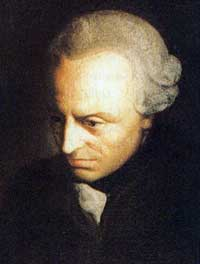
\includegraphics[height=4cm]{../../../graphics/kant.jpg}
            \end{column}
            \begin{column}{7cm}
                ``We can only learn to philosophize, that is, to exercise the talent of reason, in accordance with its universal principles, on certain actually existing attempts at philosophy, always, however, reserving the light of reason to investigate, to confirm, or to reject these principles in their very sources.''
            \end{column}
        \end{columns}
}

We will begin with Book \textsc{iii} of David Hume's \emph{Treatise of Human Nature}. I recommend the David Fate Noron edition published by Oxford University Press which is widely regarded as the authoritative edition of this text. References to the \emph{Treatise} are give by a sequence of numbers such as: \emph{Treatise} 2.3.3.2. This means \emph{Treatise} Book \textsc{ii}, Part 3, Section 3, Paragraph 2. In general, the first number of the sequence is the book, the second number is the part, the third number is the section, and the fourth number is the paragraph (sometimes paragraphs will be omitted). We this convention in mind, we will be reading the following portions of the \emph{Treatise}:
\begin{itemize}
    \item \alert{Introduction}
    \item \alert{1.1.1--5}
    \item \alert{2.1.1--5}
    \item \alert{2.1.11}
    \item \alert{2.3.3}
    \item \alert{3.1.1--2}
    \item \alert{3.2.1--3}
    \item \alert{3.3.1--6}
\end{itemize}
While mainly focusing on Book \textsc{iii}, we will go over some essential background material from Books \textsc{i} and \textsc{ii} first. \change

% \textbf{See Figure~\ref{fig:slide3}.}
% 
% \begin{figure}[ht]
%     \begin{center}
%         \includeslide[height=5cm]{slide3<1>}
%     \end{center}
%     \caption{Hume's Ethics}
%     \label{fig:slide3}
% \end{figure}

\frame<presentation>[label=slide3]{
    \frametitle{Hume's Ethics}
        \emph{A Treatise of Human Nature}, David Hume, David Fate Norton and Mary J. Norton (eds.), Oxford: Oxford University Press, 2003. The first number of the sequence is the book, the second number is the part, the third number is the section, and the fourth number is a paragraph. With this convention in mind, we will be reading the following portions of the \emph{Treatise}:
            \begin{itemize}
                \item \alert{Introduction}
                \item \alert{1.1.1--5}
                \item \alert{2.1.1--5}
                \item \alert{2.1.11}
                \item \alert{2.3.3}
                \item \alert{3.1.1--2}
                \item \alert{3.2.1--3}
                \item \alert{3.3.1--6}
            \end{itemize}
}

% section overview (end)

\section{The Project of the Treatise}\label{sec:the_project_of_the_emph_treatise_} % (fold)

The subtitle of the \emph{Treatise} is ``Being an Attempt to Introduce the Experimental Method of Reasoning into Moral Subjects''. This is revealing. Inspired by the success of Newton’s new science (due in large part to the deployment of the experimental method that Bacon prescribed), Hume endeavored to introduce the experimental method into philosophy. Just as the deployment of experimental method in \emph{natural philosophy} (by which Hume understands mechanics and astronomy and the study of nature more generally) yielded positive results, Hume believed that the deployment of experimental method in \emph{moral philosophy} (by which Hume understands the study of humans and human activity) would yield positive results as well.

Hume believed that the introduction of the experimental method into philosophy and the establishment of the ``science of human nature'' was necessary in order to resolve persistent and apparently fruitless disagreements in philosophy:
\begin{quote}
    There is nothing which is not the subject of debate, and in which men of learning are not of contrary opinions. The most trivial question escapes not our controversy, and in the most momentous we are not able to give any certain decision. Disputes are multiply’d as if everything was uncertain; and these disputes are manag’d with the greatest warmth, as if every thing was certain. (\emph{Treatise}, Intro, 2)
\end{quote}

Instead of pursuing these debates directly, Hume believed that progress could be made if we first become ``thouroughly acquainted with the extent and force of human understanding'' (\emph{Treatise}, Intro, 4). To do so we should ``explain the nature of the ideas we employ, and of the operations we perform in our reasonings'' (\emph{Treatise}, Intro, 4). It is only once we understand the origin of our ideas that we can understand what we can reasonably expect to know about other subject matters. It is in this sense that Hume describes moral philosophy or the science of human nature as the ``capital of the sciences''.

The new natural philosophy, given its experimental method, is based on observation, but it is no mere summary of these observations. The natural philosopher may legitimately generalize his observations. Moreover, natural philosophy aspires to establish a limited number of principles that can explain the greatest number of observed phenomena. Similarly, moral philosophy is to be based on observation, but is no mere summary of these observations. The moral philosopher may legitimately generalize his observations. Moreover, the moral philosopher aspires to establish a limited number of principles that can explain the greatest number of observed phenomena:
\begin{quote}
    \ldots we must endeavour to render all our principles as universal as possible, by tracing up our experiments to the utmost, and explaining all effects from the simplest and fewest causes… (\emph{Treatise}, Intro, 8)
\end{quote}
Though the natural and moral philosopher may generalize their observations in an attempt to discover fundamental and comprehensive principles, they cannot hope to transcend experience to discover the ultimate supersensible causes of things:
\begin{quote}
    \ldots 'tis still certain we cannot go beyond experience; and any hypothesis, that pretends to discover the ultimate original qualities of human nature, ought at first to be rejected as presumptuous and chimerical. (\emph{Treatise}, Intro, 8)
\end{quote}

Though both natural and moral philosophy are to be based on the experimental method, there is a crucial methodological difference between these intellectual disciplines. The natural philosopher can ``interrogate nature'' as Bacon prescribed. The natural philosopher can conduct experiments under controlled conditions ``purposely, with premeditation, and after such a manner as to satisfy itself concerning every particular difficulty which may arise''. However, in moral philosophy no such interrogation is possible. The moral philosopher cannot conduct experiments under controlled conditions. Rather, he is limited to ``a cautious observation of human life, and take them as they appear in the common course of the world, by men’s behaviour in company, in affairs and in their pleasures''. Nevertheless, such cautious observations are sufficient ``to establish \ldots\ a science, which will not be inferior in certainty, and will be much superior in utility to any other human comprehension'' (\emph{Treatise}, Intro, 10). \change

% \textbf{See Figure~\ref{fig:slide4}.}
% 
% \begin{figure}[ht]
%     \begin{center}
%         \includeslide[height=5cm]{slide4<1>}
%     \end{center}
%     \caption{The Project of the Treatise}
%     \label{fig:slide4}
% \end{figure}

\frame<presentation>[label=slide4]{
    \frametitle{The Project of the \emph{Treatise}}
        \begin{columns}
            \begin{column}{3cm}
                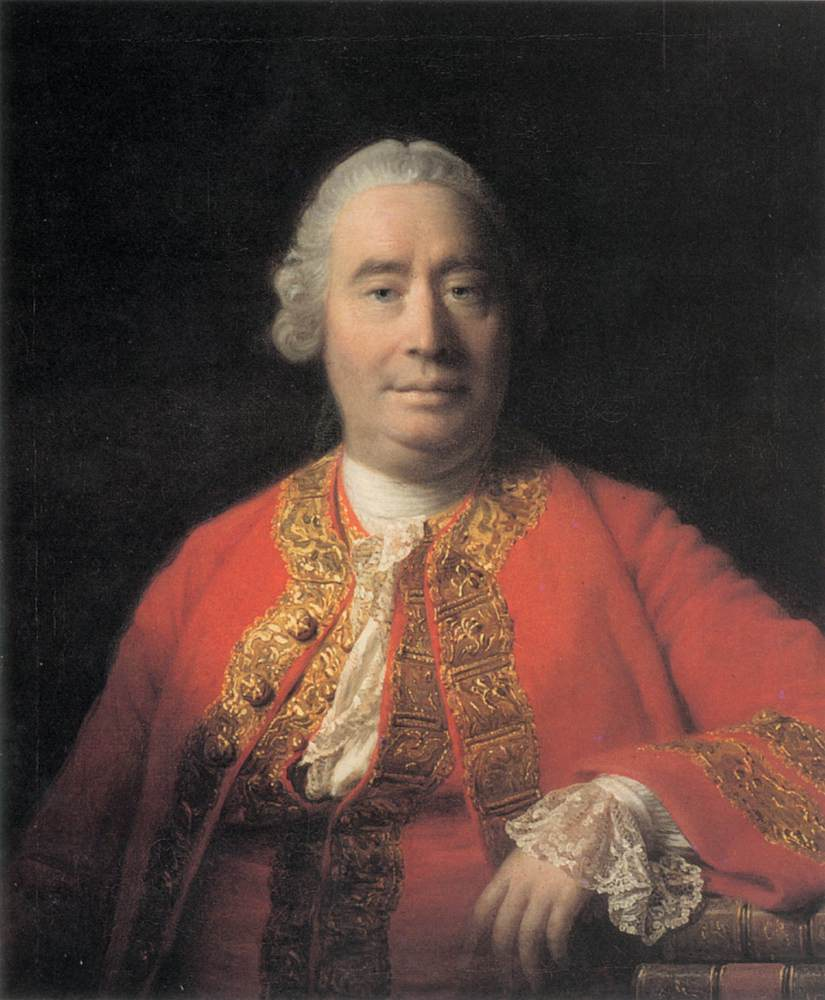
\includegraphics[height=4cm]{../../../graphics/hume.jpg}
            \end{column}
            \begin{column}{7cm}
                \begin{itemize}
                    \item Natural Philosophy \& Moral Philosophy
                    \item The Capital of the Sciences
                \end{itemize}
            \end{column}
        \end{columns}
}

A central goal of the \emph{Treatise} is to examine the origin of certain kinds of ideas and impressions. Book I discusses the origin of certain important ideas (of space and time, necessary connection, of external objects, and the self). Book II discusses the origin of certain impressions of reflections (the passions, desires, and the will). Book III discusses the origin of moral distinctions such as between vice and virtue. Hume will argue that moral distinctions depend on certain impressions.

Hume’s project in moral philosophy is primarily \emph{descriptive} and \emph{explanatory}, as opposed to being \emph{prescriptive} and \emph{justificatory}. Hume does not seek to prescribe certain moral judgments. Common morality is fine as it stands (though perhaps susceptible to certain refinements and extensions). Rather Hume seeks to describe how we come to make the moral judgments that we make. Hume seeks to explain the origin of our moral distinctions rather than to justify these distinctions (though Hume believes that once we recognize the proper explanation of the moral distinctions that we make, we will be all the more pleased to make them). Moreover, and importantly, Hume seeks to provide a \emph{naturalistic} explanation of our moral distinctions. Hume seeks to give an account of human morality as a natural phenomena---as arising from human nature and our place in nature. He thus rejects any attempt to give a theological foundation to morality of a kind that natural law theorists (such as Locke and Puffendorf) recommended.

Hutcheson famously complained that Hume’s moral science lacked sufficient ``Warmth in the Cause of Virtue''. The moral philosopher, Hume responded, must consider the human mind that gives rise to moral distinctions:
\begin{quote}
    \ldots either as an Anatomist or as a Painter; either to discover its most secret Springs \& Principles or to describe the Grace \& Beauty of its Actions. I imagine it impossible to conjoin these two Views. Where you pull off the Skin, \& display all the minute Parts, there appears something trivial, even in the noblest Attitudes \& most vigorous Actions: Nor can you ever render the object graceful or engaging but by the cloathing the Parts again with Skin \& Flesh, \& presenting only their bare Outside. An Anatomist, however, can give very good Advice to a Painter or Statuary: And in like manner, I am perswaded, that a Metaphysician may be very helpful to a Moralist; tho' I cannot easily conceive these two Characters united in the same Work. Any warm Sentiment of Morals, I am afraid, would have the Air of Declamation amidst abstract Reasonings, \& wou'd be esteem’d contrary to good Taste. And tho' I am much more ambitious of being esteem'd a Friend of Virtue, than a Writer of Taste; yet I must always carry the latter in my Eye, otherwise I must despair of ever being servicable to Virtue. (Letter of 17 September, 1739)
\end{quote}
An attitude that is perhaps reflected in the epigram of Book III:
\begin{quote}
    Dur\ae\ semper virtutis amator, Qu\ae re est virtus, et posce exemplar honesti.
    
    A lover of austere virtue, you should at least ask now what Virtue is and demand to see Goodness in her visible shape. (Lucan, \emph{Civil Wars} 9.562-3)
\end{quote}

\change

% \textbf{See Figure~\ref{fig:slide5}.}
% 
% \begin{figure}[ht]
%     \begin{center}
%         \includeslide[height=5cm]{slide5<1>}
%     \end{center}
%     \caption{The Anatomist of Morals}
%     \label{fig:slide5}
% \end{figure}

\frame<presentation>[label=slide5]{
    \frametitle{The Anatomist of Morals}
        \begin{columns}
            \begin{column}{3cm}
                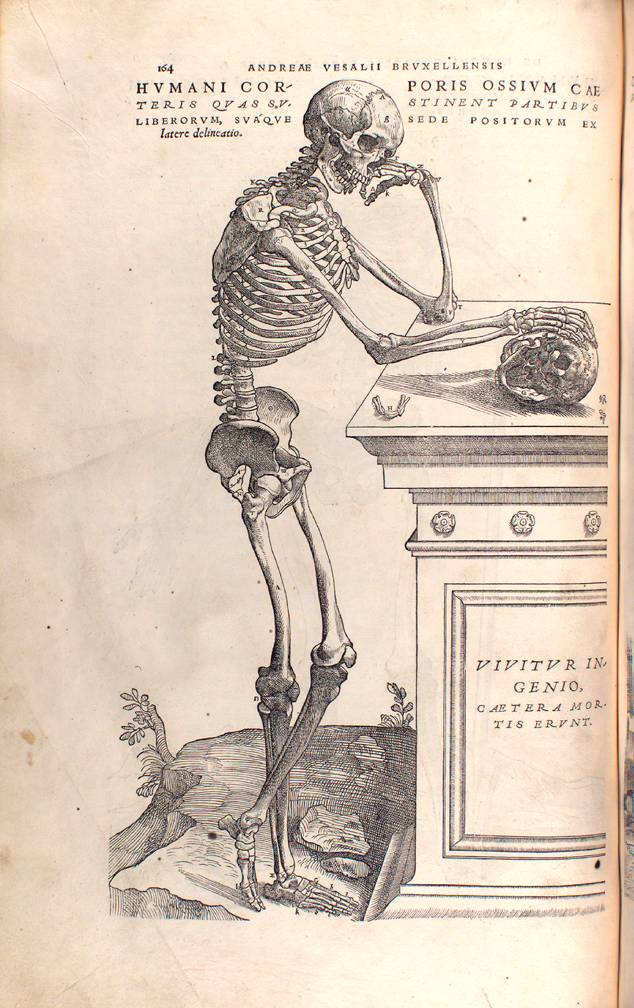
\includegraphics[height=6cm]{../../../graphics/anatomy.jpg}
            \end{column}
            \begin{column}{7cm}
                \begin{itemize}
                    \item Hume's moral philosophy is \alert{descriptive} \& \alert{explanatory} as opposed to \alert{prescriptive} and \alert{justificatory}
                    \item Hume aims to provide a \alert{naturalistic} as opposed to a \alert{theological} foundation for morality
                \end{itemize}
            \end{column}
        \end{columns}
}

% section the_project_of_the_emph_treatise_ (end)

\section{Hume's Philosophical Psychology}\label{sec:hume_s_psychology} % (fold)

Book I of the \emph{Treatise} ends on a note of despair:

\begin{quote}
    But before I launch out into these immense depths of philosophy, which lie before me, I find myself inclin’d to stop a moment in my present station, and to ponder that voyage, which I have undertaken, and which undoubtedly requires the utmost art and industry to be brought to a happy conclusion. Methinks I am like a man, who having struck on many shoals, and having narrowly escap'd shipwreck in passing a small frith, has yet the temerity to put out to sea in the same leaky weather-beaten vessel, and even carries his ambition so far as to think of compassing the globe under these disadvantageous circumstances. \ldots And the impossibility of amending or correcting these faculties, reduces me almost to despair, and makes me resolve to perish on the barren rock, on which I am present, rather than venture myself upon the boundless ocean, which runs out into immensity. (\emph{Treatise}, 1.4.7.1)
\end{quote}

What Hume despairs of is the possibility of reasonable metaphysical speculation about the supersensible nature of things---for example, about the nature of the necessary connection between cause and effect. If philosophy cannot reasonably engage in such metaphysical speculation, what is there left for philosophy to do?

Hume's skepticism, however, is merely limited to metaphysical speculation about the supersensible nature of things. Philosophy may not reasonable engage in such speculation, but, through cautious observation, philosophy may nevertheless investigate human nature. Hume's theory of the passions exemplifies what can be done in the new science of human nature, for certain passions, the indirect passions, are governed by a limited number of general principles that can be discovered by cautious observation of humans and human activity. \change

% \textbf{See Figure~\ref{fig:slide6}.}
% 
% \begin{figure}[ht]
%     \begin{center}
%         \includeslide[height=5cm]{slide6<1>}
%     \end{center}
%     \caption{Hume's Despair}
%     \label{fig:slide6}
% \end{figure}

\frame<presentation>[label=slide6]{
    \frametitle{Hume's Despair}
        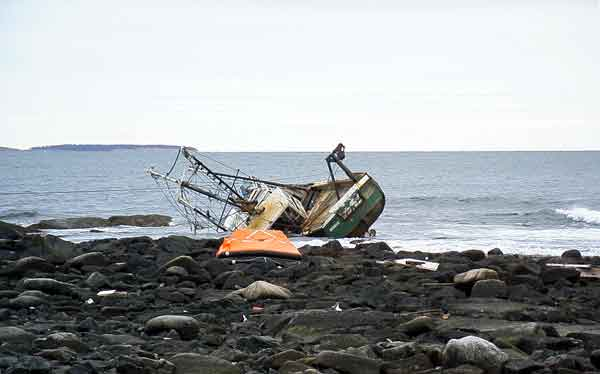
\includegraphics[width=\textwidth]{../../../graphics/shipwreck.jpg}
}

Hume calls whatever is present to the mind \emph{perceptions}: ``all the actions of seeing, hearing, judging, loving, hating, and thinking, fall under this denomination'' (\emph{Treatise}, 3.1.1.2). \change\ There are two kinds of perceptions, \emph{impressions} and \emph{ideas}. Impressions enter the mind with greater force or vivacity than ideas, the ``faint images'' of impressions. \change

Impressions and ideas are either simple or complex. Simple perceptions, such as impressions of particular colors, ``admit of no distinction nor separation''. In contrast, complex perceptions, impressions or ideas of Paris, say, are such that constituent parts can be distinguished. Our impressions of Paris include the distinguishable sights and sounds of that city. \change

% \textbf{See Figure~\ref{fig:slide7}.}
% 
% \begin{figure}[ht]
%     \begin{center}
%         \includeslide[height=5cm]{slide7<3>}
%     \end{center}
%     \caption{Perceptions in the Mind}
%     \label{fig:slide7}
% \end{figure}

\frame<presentation>[label=slide7]{
    \frametitle{Perceptions in the Mind}
        \begin{columns}
            \begin{column}{3cm}
                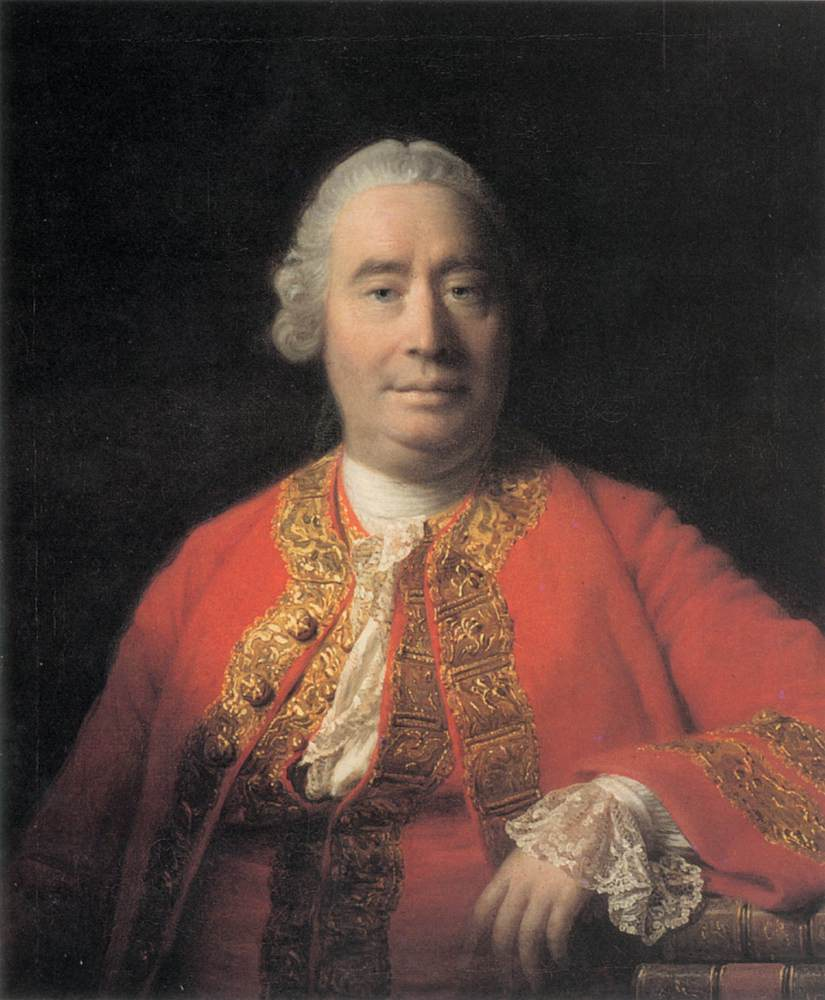
\includegraphics[height=4cm]{../../../graphics/hume.jpg}
            \end{column}
            \begin{column}{7cm}
                \begin{itemize}
                    \item<1-> The immediate objects of the mind are \alert{perceptions}
                    \item<2-> Perceptions are either \alert{impressions} or \alert{ideas}
                    \item<3-> Impressions and ideas are either \alert{simple} or \alert{complex}
                \end{itemize}
            \end{column}
        \end{columns}
}

While Hume initially distinguishes impressions and ideas in terms of the force or vivacity by which they enter the mind, he makes the further important claim that simple ideas are causally dependent on impressions that resemble them. (And since complex ideas depend on the simple ideas that are their constituents, complex ideas ultimately depend as well on the simple impressions from which their constituent simple ideas derive. Hume describes this as ``the first principle in the science of human nature'':

\begin{quote}
    \ldots that all our simple ideas in their first appearance are deriv'd from simple impressions, which are correspondent to them, and which they exactly represent. (\emph{Treatise}, 1.1.1.7)
\end{quote}

Our ideas of particular colors \emph{resemble} the impressions of those particular colors: ``The idea of red, which we form in the dark, and that impression, which strikes our eyes in sun-shine, differ only in degree, not in nature'' (\emph{Treatise}, 1.1.1.5). Moreover our ideas of particular colors \emph{causally depend} on our impressions of them: ``To give a child an idea of scarlet or orange,of sweet or bitter, I present the objects, or in other words, convey to him these impressions; but proceed not so absurdly, as to endeavour to produce the impressions by exciting the ideas'' (\emph{Treatise}, 1.1.1.8) Putting these two claims together we get Hume's first principle of the science of human nature. The support for this important claim is limited to ``cautious observation'' that simple ideas invariably derive from simple impressions that resemble them. \change

% \textbf{See Figure~\ref{fig:slide8}.}
% 
% \begin{figure}[ht]
%     \begin{center}
%         \includeslide[height=5cm]{slide8<1>}
%     \end{center}
%     \caption{The First Principle in the Science of Human Nature}
%     \label{fig:slide8}
% \end{figure}

\frame<presentation>[label=slide8]{
    \frametitle{The First Principle in the Science of Human Nature}
        \ldots that all our simple ideas in their first appearance are deriv'd from simple impressions, which are correspondent to them, and which they exactly represent. (\emph{Treatise}, 1.1.1.7)
}

Hume observes that there are two kinds of impressions: \emph{impressions of sensation} and \emph{impressions of reflection} (\emph{Treatise}, 1.1.2).

Impressions of sensation include colors, taste, smell, etc., as well as pains and pleasures. Impressions of sensation derive ``in the soul originally, from unknown causes''. This is all that Hume ever says about the origins of impressions of sensations. This is because discovering the cause of impressions of sensations is the task of a specific sub-discipline of natural philosophy, i.e., speculative anatomy, and Hume is concerned only with moral philosophy, the science of human nature.

Impressions of reflection include passions, desires, and emotions. Whereas impressions of sensations are \emph{original impressions} in the sense that experience begins with them, impressions of reflection are \emph{secondary impressions} in the sense that they are ``deriv’d in a great measure from our ideas''. We initially experience certain original impressions. These give rise to certain ideas that resemble them. These in turn can give rise to further impressions. These are the impressions of reflection. Thus, for example, I can experience the smell of rotten eggs. This impression is disagreeable and causes me pain. On the basis of my impression, I form an idea of the smell of rotten eggs. This idea in turn gives rise to a feeling of aversion, a strong inclination to avoid smelling rotten eggs again. This new feeling of aversion is an impression of reflection. \change

% \textbf{See Figure~\ref{fig:slide9}.}
% 
% \begin{figure}[ht]
%     \begin{center}
%         \includeslide[height=5cm]{slide9<1>}
%     \end{center}
%     \caption{Perceptions in the Mind}
%     \label{fig:slide9}
% \end{figure}

\frame<presentation>[label=slide9]{
    \frametitle{Perceptions in the Mind}
        \begin{center}
        	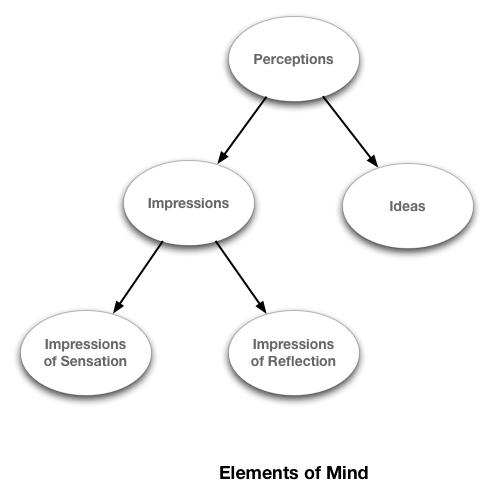
\includegraphics[height=7cm]{../../../graphics/perceptions.jpg}
        \end{center}
        
}

In the \emph{Treatise}, Hume seeks to describe the origin of certain impressions and ideas and the operations upon them. In describing ``the connexion or association of ideas'' Hume distinguishes two kinds of relations: \emph{natural} and \emph{philosophical}.

There are three natural relations:

\begin{itemize}
    \item Resemblance
    \item Contiguity
    \item Causation
\end{itemize}

For example, if we see a portrait of Locke (pictured here), this might lead us to think of the philosopher that it resembles. Similarly, if we see 10 Downing Street, this might lead us to think of the prime minister who (while in residence at least) is contiguous with it. Similarly, if we experience a certain effect, this might lead us to think of its cause. So, if see wet pavement on a sunny day, this might lead us to think of the recent rain that caused it. In each case there is an ``associating quality'' which connects two ideas in such a way that entertaining either idea ``naturally introduces the other'' (\emph{Treatise}, 1.1.5.1).

According to Hume, these relations produce ``unity or cohesion'' among our ideas. Ideas that are related by resemblance, contiguity, or causation are naturally associated as if by a force analogous to gravity or magnetism. It is in this sense that Hume describes them as ``the cement of the universe''. Of course, by means of our imagination we can conjoin any two ideas we wish, but even here, in virtue of the force of natural association between particular ideas we are inclined to associate them in imagination more frequently than ideas that are not naturally associated or are naturally associated to a lesser degree. \change

% \textbf{See Figure~\ref{fig:slide10}.}
% 
% \begin{figure}[ht]
%     \begin{center}
%         \includeslide[height=5cm]{slide10<1>}
%     \end{center}
%     \caption{The Connexion or Association of Ideas}
%     \label{fig:slide10}
% \end{figure}

\frame<presentation>[label=slide10]{
    \frametitle{The Connexion or Association of Ideas}
        \begin{columns}
            \begin{column}{3cm}
                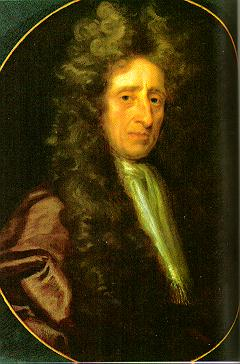
\includegraphics[height=4cm]{../../../graphics/locke.jpg}
            \end{column}
            \begin{column}{7cm}
                \alert{Natural Relations}:
                    \begin{itemize}
                        \item Resemblance
                        \item Contiguity
                        \item Causation
                    \end{itemize}
            \end{column}
        \end{columns}
}


% By means of the imagination we can associate any two ideas whatsoever. When we do so, we can ask how they are related. In this manner, we produce the ``ideas of philosophical relation''. There are seven philosophical relations:
% 
% \begin{itemize}
%     \item Resemblance
%     \item Identity
%     \item Space and time
%     \item Proportions in quantity or number
%     \item Degree in any quality
%     \item Contrariety
%     \item Causation
% \end{itemize}
% 
% In calling such relations \emph{philosophical} relations, perhaps, Hume is suggesting that such imaginative comparisons is essential to philosophical inquiry.

% section hume_s_psychology (end)

\section{Next Time}\label{sec:summary} % (fold)

% \textbf{See Figure~\ref{fig:slide11}.}
% 
% \begin{figure}[ht]
%     \begin{center}
%         \includeslide[height=5cm]{slide11<1>}
%     \end{center}
%     \caption{Readings for Next Time}
%     \label{fig:slide11}
% \end{figure}


\frame<presentation>[label=slide11]{
    \frametitle{Readings for Next Time}
        Covered this lecture:
            \begin{itemize}
                \item Treatise, \alert{Introduction}
                \item Treatise, \alert{1.1.1--5}
            \end{itemize}
        Covered next lecture:
            \begin{itemize}
                \item Treatise, \alert{2.1.1–5}
                \item Treatise, \alert{2.1.11}
            \end{itemize}
        Optional Reading:
            \begin{itemize}
                \item Rawls, \alert{Introduction}, \alert{Hume I}, \alert{Hume II}
                \item Wiggins, \alert{Chapter 1}, \alert{Chapter 2}
            \end{itemize}
}

% section summary (end)

\end{document}
